\documentclass[12pt]{article}
\usepackage{fullpage, subfig}
\usepackage{mathtools, lipsum, url}
\usepackage[a4paper,top=2.5cm,bottom=2.5cm,left=2.5cm,right=2.5cm,marginparwidth=1.75cm]{geometry}
\usepackage{amsmath}
\usepackage{graphicx, float}
\usepackage[dvipsnames]{xcolor}
\linespread{1.3}
\usepackage{natbib}
\usepackage[hidelinks,colorlinks=true,linkcolor=blue,citecolor=blue]{hyperref}
\usepackage{caption}
\usepackage{subcaption}


\title{How do mental health medications impact the Body Mass Index?}
\author{Group 090}
\date{}

\begin{document}
\maketitle

\section{Introduction}

 This project explores the impact of prescribed mental health medications (antidepressants, antipsychotics, and hypnotics) on the body mass index (BMI) of individuals suffering from mental illnesses. While current literature suggests that usage of such medication could lead to increases in BMI, some studies offer conflicting evidence and unclear relationships \citep{ ALBERICH2019112506}. Using data from the 2019 Health Survey for England, our goal was to investigate the impacts of mental health medication on the Body Mass Index of both males and females. We chose this iteration of the survey because it was the most recent publicly available dataset before the COVID-19 pandemic, as datasets from 2020 and onwards might distort the results of our study. \\
 

\noindent 
As part of our study, we considered the following variables: 

\begin{enumerate}
    
    \item Valid BMI (5 groups) estimated weight if $>200$ kg

   \item Any prescribed mental health 
medications taken in last 7 days

    \item Any prescribed Hypnotics medications taken in last 7 days

    \item Any prescribed Antipyschotic medications taken in last 7 days

    \item Any prescribed Antidepressants medications taken in last 7 days

    \item Sex
\end{enumerate}

10299 people participated in the survey. After data filtration, we considered 4358 observations. Of which, 2437 are females, and 1921 are males. Amongst males, 163 were prescribed some form of mental health medication. For females, 388 were prescribed medication. 14 people were prescribed only antipsychotics, 16 were prescribed only hypnotics and 471 were prescribed only antidepressants.



\section{Data Analysis}

We 	hypothesised that the BMI would be higher amongst those who were taking mental health medication. Mental health medications interfere with hormonal balances, potentially disturbing metabolic processes, eating habits and energy, leading to lower physical exercise and higher calorie intake \citep{Mazereel2020}. While \cite{Mazereel2020} is a thorough review of existing literature, we ran this study to verify whether this relationship was regionally applicable to England. We would also like to explore whether taking mental health medication causes high BMI. However, we are only able to study correlations.

%(they used old dataset/wanted to check if it was regionally appplicable to the UK)



\begin{figure}[h]
    \centering
    
    \begin{minipage}{0.49\textwidth}
    \centering
    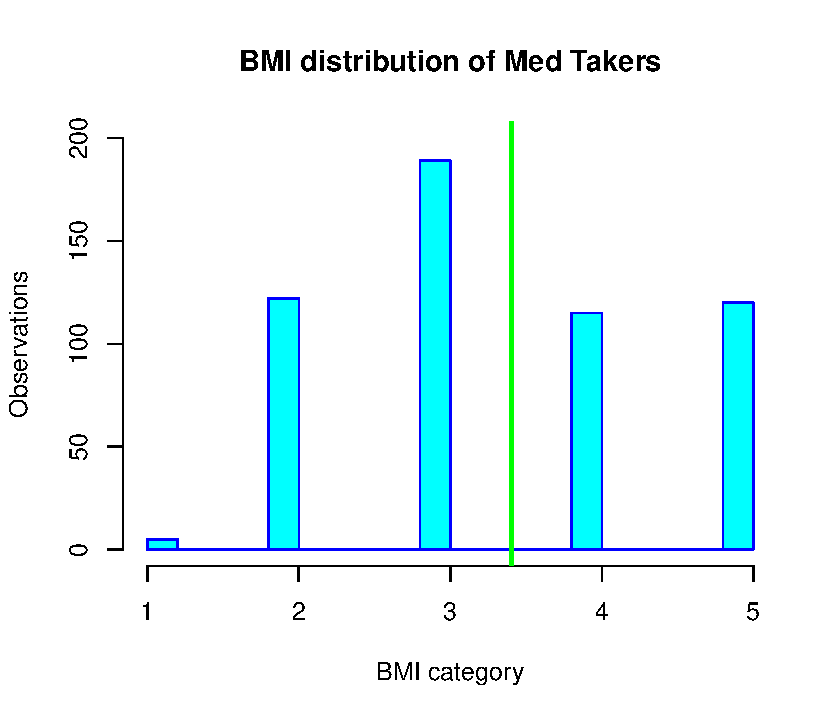
\includegraphics[width=1\textwidth]{rplots/Rplot.pdf}
    \caption{}
    \label{fig:bmidistmed}
    \end{minipage}
    \hfill
    \begin{minipage}{0.49\textwidth}
    \centering
    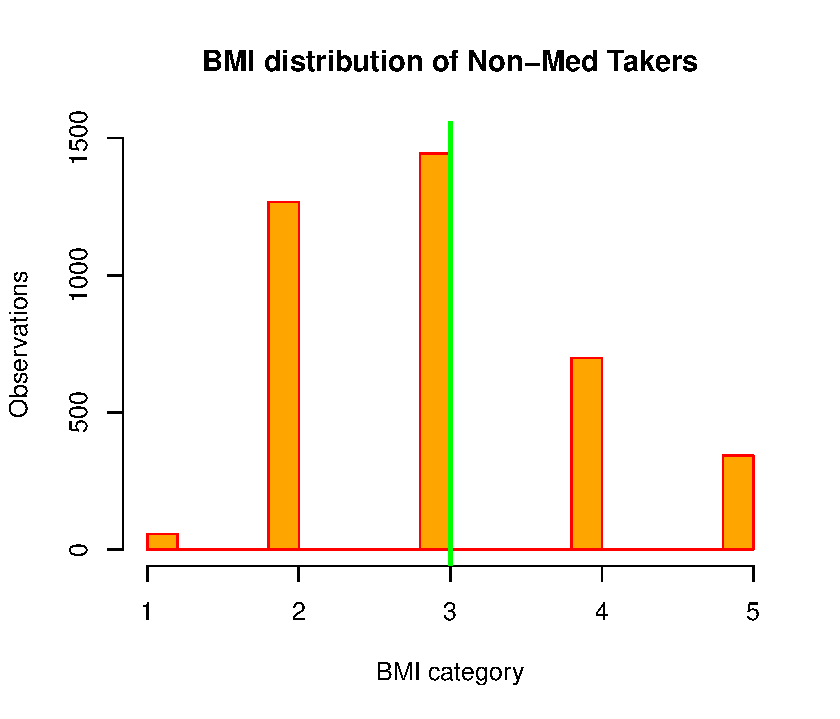
\includegraphics[width=1\textwidth]{rplots/Rplot01.pdf}
    \caption{}
    \label{fig:bmidistnonmed}
    \end{minipage}
    
\end{figure}

 At first glance, the hypothesis that BMI is correlated to mental health medication intake seems to be confirmed. Our findings in Figures \ref{fig:bmidistmed} and \ref{fig:bmidistnonmed} show the mean BMI of the general sample, with a mean of 3.0 for non-medicine takers, compared to the mean of 3.4 for medicine takers. Even though the difference in means is 0.4, we need to find if it is statistically significant. \\
 
 Within the independent samples of mental health medicine takers and non-takers, we conducted the following hypothesis test on the difference in mean Body Mass Index of the two groups:
\begin{equation}
    \begin{split} \label{hypothesis}
        H_0 :	\mu_{\text{MED}}-\mu_{\text{NoMED}} = 0 \\
        H_1 :	\mu_{\text{MED}}-\mu_{\text{NoMED}} > 0
    \end{split}
    \end{equation}

 We approximated the underlying distributions by the normal according to the Central Limit Theorem and assumed equal population variance. Subsequently, we ran a one-tailed t-test with a significance level of 1 per cent and rejected the null hypothesis. \\

 According to existing literature, the relative magnitude of mental health medication-related weight gain is dependent, to an extent, on biological sex. \cite{Gates2016} states that women gained significantly more weight. To test the validity of this conclusion, we then tested for sex-based differences  in the BMI distributions.

\begin{figure}[h]
    \centering
    
    \begin{minipage}{0.49\textwidth}
    \centering
    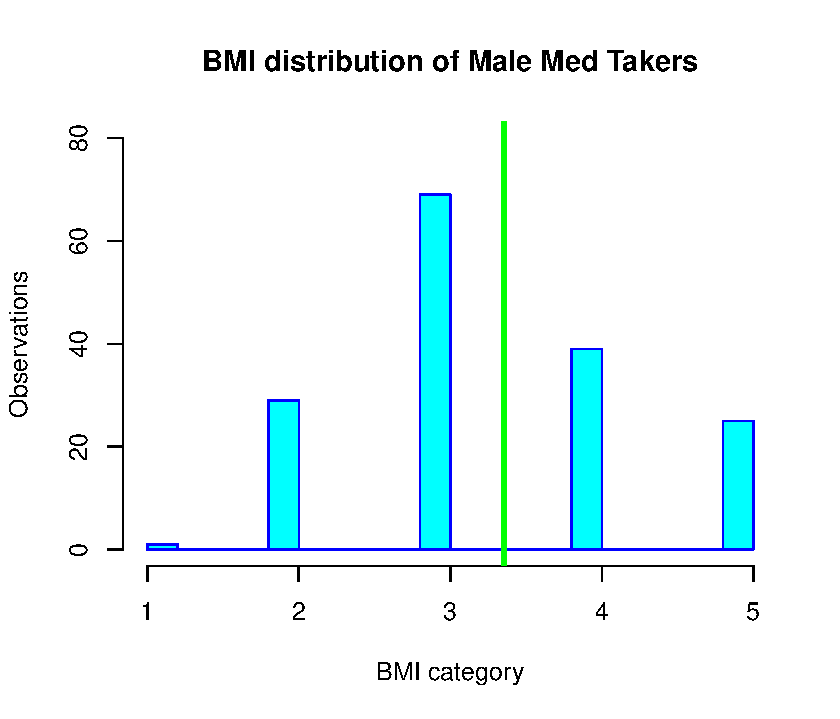
\includegraphics[width=1\textwidth]{rplots/Rplot02.pdf}
    \caption{}
    \label{fig:bmidistmedmale}
    \end{minipage}
    \hfill
    \begin{minipage}{0.49\textwidth}
    \centering
    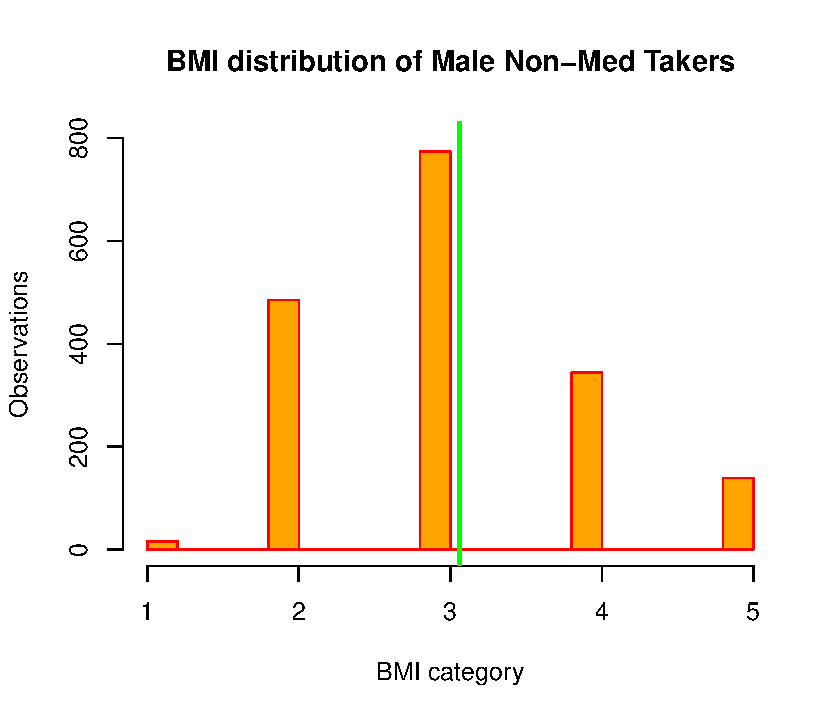
\includegraphics[width=1\textwidth]{rplots/Rplot03.pdf}
    \caption{}
    \label{fig:bmidistnonmedmale}
    \end{minipage}
    
\end{figure}

Figures \ref{fig:bmidistmedmale} and \ref{fig:bmidistnonmedmale} compare the mean BMI of male medicine takers, with a mean of 3.35 and the mean BMI of male non-medicine takers at 3.06. 
\begin{figure}[h]
    \centering
    
    \begin{minipage}{0.49\textwidth}
    \centering
    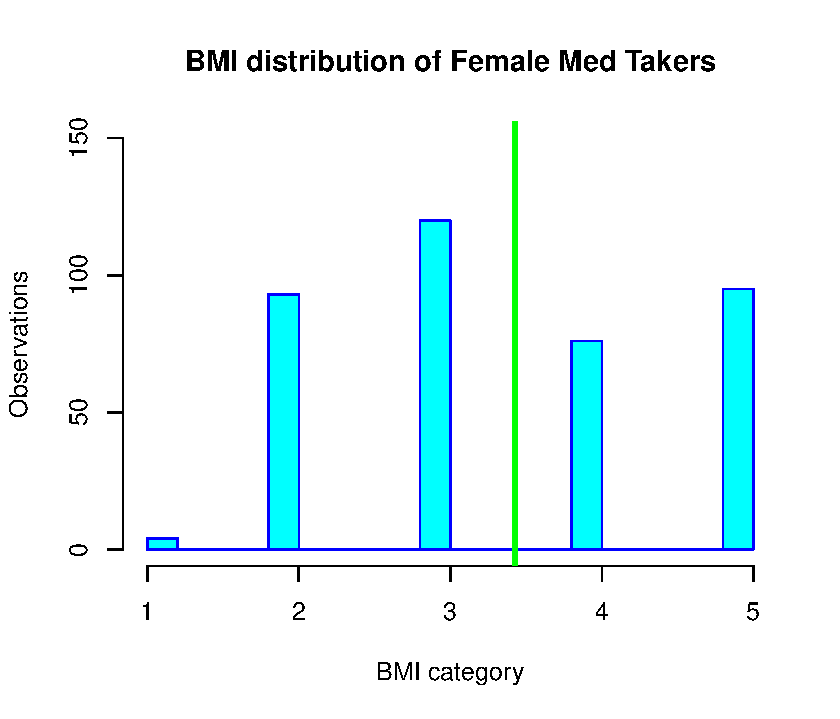
\includegraphics[width=1\textwidth]{rplots/Rplot04.pdf}
    \caption{}
    \label{fig:bmidistmedfemale}
    \end{minipage}
    \hfill
    \begin{minipage}{0.49\textwidth}
    \centering
    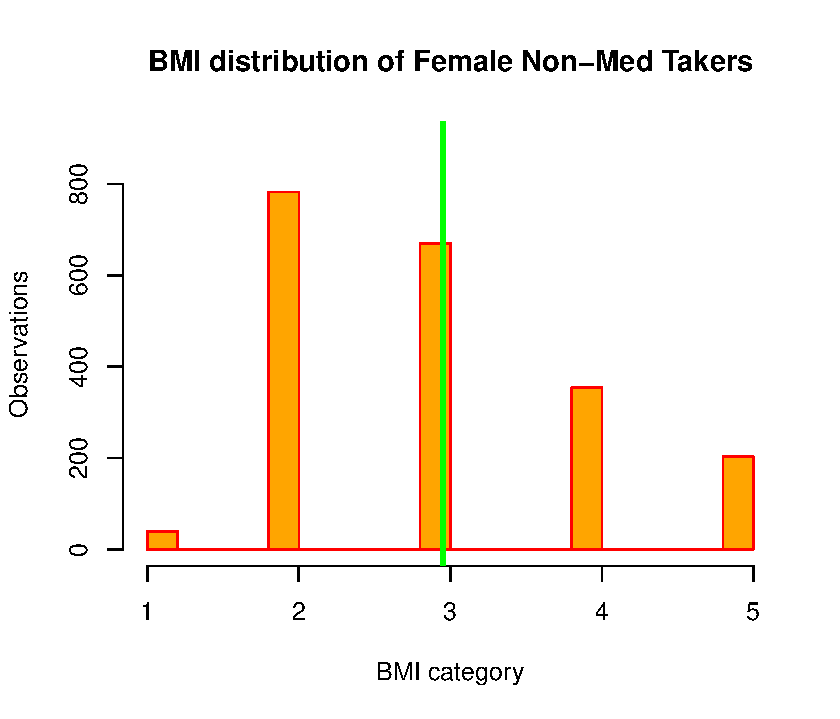
\includegraphics[width=1\textwidth]{rplots/Rplot05.pdf}
    \caption{}
    \label{fig:bmidistnonmedfemale}
    \end{minipage}
    
\end{figure} \\


\newpage

Figures \ref{fig:bmidistmedfemale} and \ref{fig:bmidistnonmedfemale} compare the mean BMI of female medicine takers, with a mean of 3.43, compared to the mean BMI of female non-medicine takers at 2.95. The analysis reveals a difference in means of 0.29 for males and 0.48 for females. We had to test these differences in means to determine their statistical significance. We ran a two-tailed t-test of the male medicine takers' BMI means against the means of the female medicine takers' BMI. With an insignificant p-value, we failed to reject the null hypothesis at the 5 per cent significance level.
\\
\begin{equation}
    \begin{split}
        H_0 :	\mu_{\text{MaleMED}}-\mu_{\text{FemaleMED}} = 0 \\
        H_1 :	\mu_{\text{MaleMED}}-\mu_{\text{FemaleMED}} \neq 0
    \end{split}
    \end{equation}\\

To make our investigation more robust, we then analysed the weight gain related to three types of mental health medication (antidepressants, antipsychotics and hypnotics). \cite{Vanina2002} demonstrates statistically significant differences in weight gain associated with each type of medication, as does \cite{mahli}. Hence, we investigated this relationship to determine which type of medication was linked to the greatest weight gain and if the results found in these studies still hold today as medications have changed.

\begin{figure}[h]
    \centering
    
    \begin{minipage}{0.32\textwidth}
    \centering
    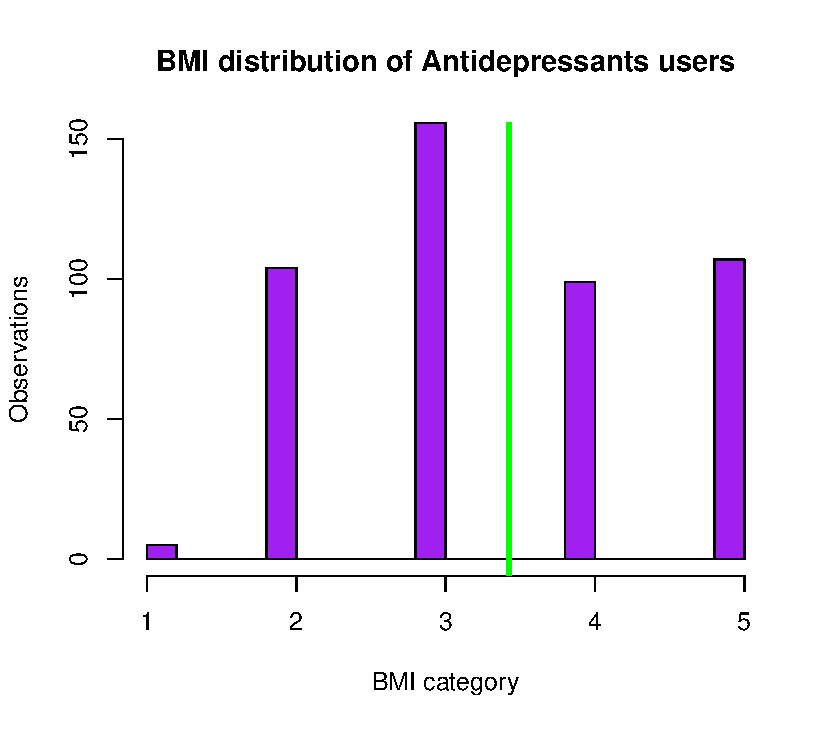
\includegraphics[width=1\textwidth]{rplots/RplotAntiDep.pdf}
    \caption{}
    \label{fig:antidep}
    \end{minipage}
    \hfill
    \begin{minipage}{0.32\textwidth}
    \centering
    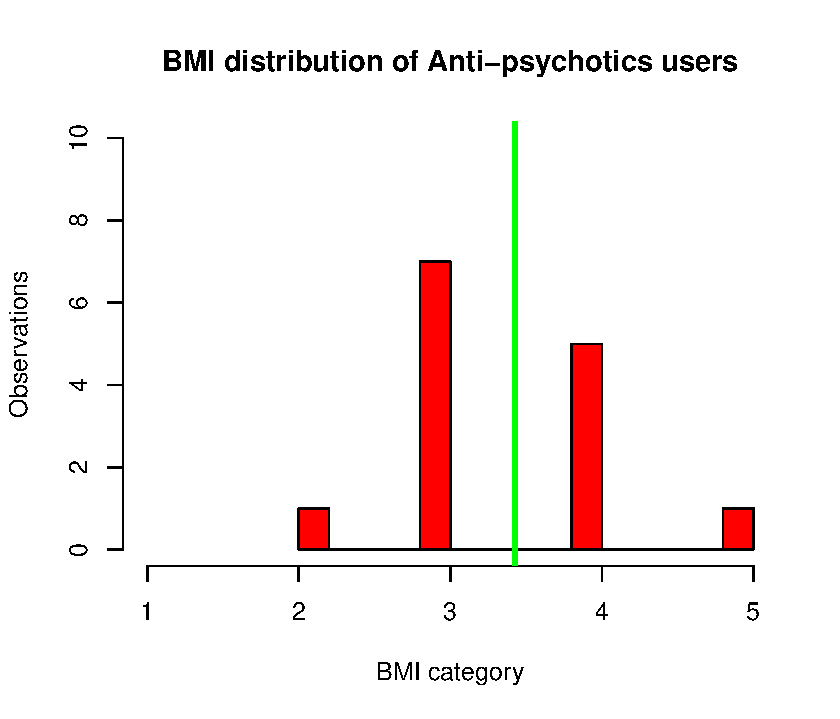
\includegraphics[width=1\textwidth]{rplots/Rplot07.pdf}
    \caption{}
    \label{fig:antipsy}
    \end{minipage}
    \hfill
    \begin{minipage}{0.32\textwidth}
    \centering
    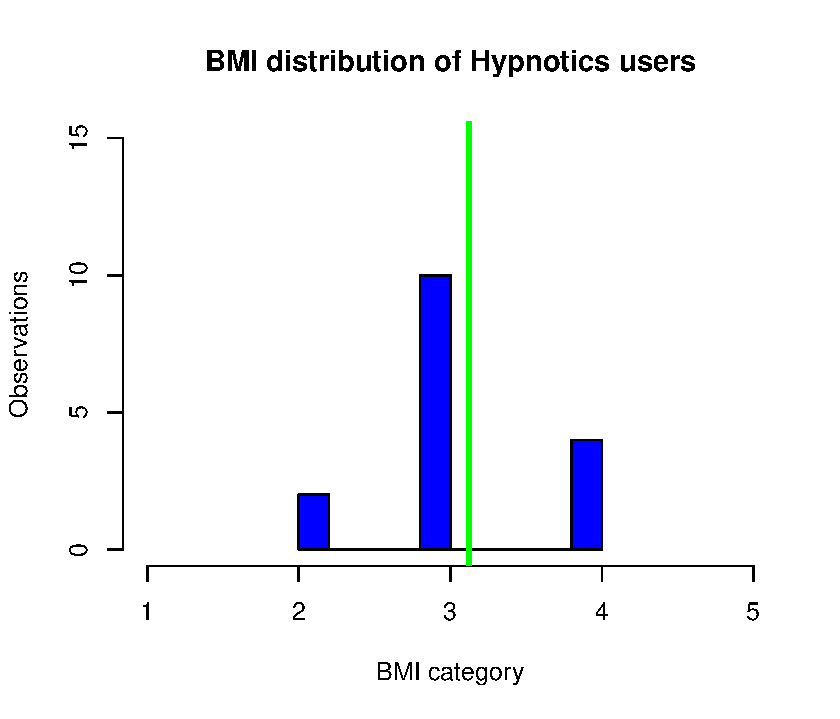
\includegraphics[width=1\textwidth]{rplots/Rplot08.pdf}
    \caption{}
    \label{fig:antihyp}
    \end{minipage}
\end{figure}


\newpage Figures \ref{fig:antidep}, \ref{fig:antipsy} and \ref{fig:antihyp} directly look at the means of people specifically on one drug, antidepressants, antipsychotics, and hypnotics respectively. The mean BMI of those only on antidepressants was 3.4, and due to small sample sizes, we also looked at the median value of 3.0. The mean BMI of people only on antipsychotics was 3.4, with a median of 3.5. The mean BMI of people only on hypnotics was 3.1, having a median of 3.0. Due to the low number of observations for each independent sample, the underlying distribution cannot be approximated with a normal. We also ran a Shapiro-Wilk normality test on all those using each type of medication, arriving at p-values less than 0.05, implying that these variables are not normally distributed. The only way to find statistical significance is through non-parametric tests of medians.
\begin{equation} 
    \begin{split}
        \label{mann_whitney_deppsy}
            H_0 :	\eta_{\text{Dep}} -\eta_{\text{Psy}} = 0 \\
            H_1 :	\eta_{\text{Dep}} - \eta_{\text{Psy}} < 0
    \end{split}
\end{equation}
\begin{equation}
    \begin{split}
     \label{mann_whitney_dephypno}
       H_0 :	\eta_{\text{Dep}}-\eta_{\text{Hypno}} = 0 \\
       H_1 :	\eta_{\text{Dep}}-\mu_{\text{Hypno}} \neq 0
    \end{split}
\end{equation}
\begin{equation} 
\begin{split}
\label{mann_whitney_psyhypno}
        H_0 :	\eta_{\text{Psy}}-\eta_{\text{Hypno}} = 0 \\
        H_1 :	\eta_{\text{Psy}}-\mu_{\text{Hypno}} > 0
        \end{split}
 \end{equation} \\


For these values, we ran three separate Mann-Whitney U tests. We found p-values: 0.45 for the difference between the medians of antidepressants and antipsychotics, 0.32 for the difference between the medians of antidepressants and hypnotics, and 0.136 for the difference between the medians of antipsychotics and hypnotics. None of these values were significant at the 5 per cent level. Therefore, we failed to reject the null hypotheses.\\

If more independent observations were available, we might find significant differences in means of at least hypnotics users and antipsychotics users that would confirm previous results showing higher weight gain from antipsychotics \citep{alonso}.



  

\newpage\section{Conclusions}

\hspace{\parindent} Our analysis of the 2019 Health Survey for England confirms our hypothesis that the use of mental health medication positively impacts an individual’s BMI. However, we fail to notice that this effect is more pronounced in females than in males and that the specific type of mental health medication used has an influence. \\

 To strengthen our present analysis, we should address the causal relationship between mental health medications and BMI through Instrumental Variable Analysis. We were restricted by small sample sizes since it is common practice to use multiple mental health medications in combination. We recognise the need for more extensive censuses and medical studies to strengthen our observations, particularly regarding the varying impact of different types of mental health medication. \\


\newpage
\bibliographystyle{agsm}
\bibliography{ref}
\end{document}